% Teaser figure -- the actual system, left to right:
%   layer weights split into crossbars -> packed into tiles (PO decides the
%   grouping) -> tiles mapped onto the 3D NoC (funnel, PF, PL) -> routing
%   choice among admissible paths.
% Standalone; pdflatex fig_crosslayer.tex -> fig_crosslayer.pdf
\documentclass[border=3pt]{standalone}
\usepackage{times}
\usepackage{tikz}
\usetikzlibrary{arrows.meta,positioning,calc}

\definecolor{cPack}{HTML}{2A78D6}   % packing
\definecolor{cMap}{HTML}{EB6834}    % mapping / PL
\definecolor{cRoute}{HTML}{1BAF7A}  % routing
\definecolor{cInk}{HTML}{101720}
\definecolor{cInk2}{HTML}{3A4653}
\definecolor{cFaint}{HTML}{9AA5B1}
\definecolor{cGridL}{HTML}{C9D2DB}

\begin{document}
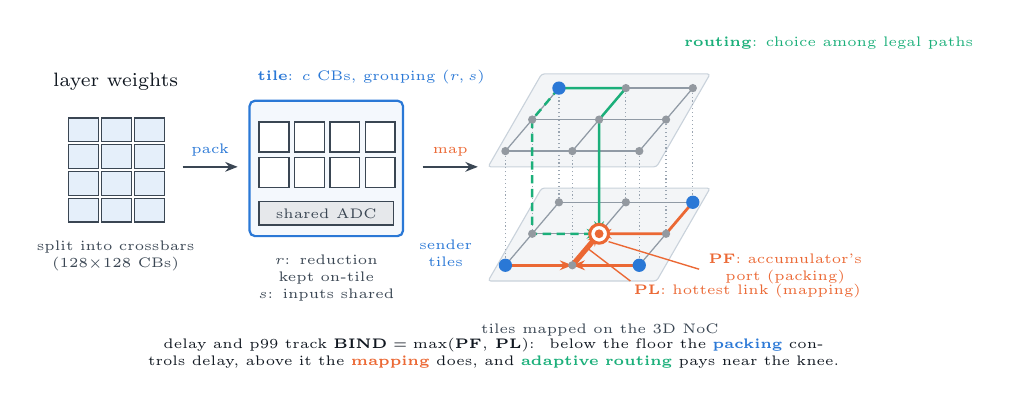
\begin{tikzpicture}[
  font=\scriptsize,
  ar/.style={-{Stealth[length=4.5pt,width=3.5pt]},line width=0.8pt,color=cInk2},
  lbl/.style={font=\scriptsize,color=cInk,align=center},
  sub/.style={font=\tiny,color=cInk2,align=center},
]

% ============================================================ A. crossbars
\begin{scope}[shift={(0,0)}]
  % layer weight matrix split into a grid of CBs
  \foreach \i in {0,1,2} \foreach \j in {0,1,2,3}
    \draw[line width=0.5pt,color=cInk2,fill=cPack!12]
      (\i*0.42,\j*0.34) rectangle ++(0.38,0.30);
  \node[lbl,anchor=south] at (0.6,1.55) {layer weights};
  \node[sub,anchor=north] at (0.6,-0.12) {split into crossbars\\(128$\times$128 CBs)};
\end{scope}

\draw[ar] (1.45,0.7) -- (2.15,0.7)
  node[midway,above,sub,color=cPack]{pack};

% ============================================================ B. the tile
\begin{scope}[shift={(2.3,-0.18)}]
  \draw[line width=0.8pt,color=cPack,rounded corners=2pt,fill=cPack!5]
      (0,0) rectangle (1.95,1.72);
  % c=8 crossbars grouped (r,s) = (2,4)
  \foreach \i in {0,1,2,3} \foreach \j in {0,1}
    \draw[line width=0.5pt,color=cInk2,fill=white]
      (0.12+\i*0.45,0.62+\j*0.45) rectangle ++(0.38,0.38);
  % row braces meaning
  \node[sub,anchor=west,color=cPack] at (-0.02,2.02)
      {\textbf{tile}: $c$ CBs, grouping $(r,s)$};
  % shared periphery strip
  \draw[line width=0.5pt,color=cInk2,fill=cFaint!25]
      (0.12,0.14) rectangle (1.83,0.44);
  \node[sub] at (0.975,0.29) {shared ADC};
  \node[sub,anchor=north,text width=24mm] at (0.975,-0.12)
      {$r$: reduction kept on-tile\\$s$: inputs shared};
\end{scope}

\draw[ar] (4.5,0.7) -- (5.2,0.7)
  node[midway,above,sub,color=cMap]{map};

% ============================================================ C. the 3D NoC
% exploded two-layer view: sheared 3x3 planes, dotted verticals
\begin{scope}[shift={(5.55,-0.55)}]
  \newcommand{\nodeat}[3]{({#1*0.85+#2*0.34},{#2*0.40+#3*1.45})}
  % layer planes (drawn first, as light parallelograms)
  \foreach \z in {0,1}
    \draw[line width=0.4pt,color=cGridL,fill=cGridL!22,rounded corners=1pt]
      ($(-0.22,-0.20+\z*1.45)$) -- ($(1.92,-0.20+\z*1.45)$) --
      ($(2.60,0.98+\z*1.45)$)  -- ($(0.46,0.98+\z*1.45)$) -- cycle;
  % vertical links (dotted, behind the in-layer links)
  \foreach \i in {0,1,2} \foreach \j in {0,1,2}
    \draw[line width=0.4pt,color=cFaint,densely dotted]
      \nodeat{\i}{\j}{0} -- \nodeat{\i}{\j}{1};
  % in-layer links
  \foreach \z in {0,1} \foreach \i in {0,1,2} \foreach \j in {0,1}{
    \draw[line width=0.45pt,color=cGridL!60!cInk2] \nodeat{\i}{\j}{\z} -- \nodeat{\i}{(\j+1)}{\z};
    \draw[line width=0.45pt,color=cGridL!60!cInk2] \nodeat{\j}{\i}{\z} -- \nodeat{(\j+1)}{\i}{\z};
  }
  % ---- the reduction funnel, Manhattan, on links -------------------------
  % two flows share (1,0,0)->(1,1,0): the hottest link (PL)
  \draw[ar,color=cMap,line width=1.0pt]
    \nodeat{0}{0}{0} -- \nodeat{1}{0}{0};
  \draw[ar,color=cMap,line width=1.0pt]
    \nodeat{2}{0}{0} -- \nodeat{1}{0}{0};
  \draw[ar,color=cMap,line width=1.9pt]
    \nodeat{1}{0}{0} -- \nodeat{1}{1}{0};
  \draw[ar,color=cMap,line width=1.0pt]
    \nodeat{2}{2}{0} -- \nodeat{2}{1}{0} -- \nodeat{1}{1}{0};
  % ---- routing choice from a top-layer source ---------------------------
  \draw[ar,color=cRoute,line width=0.9pt]
    \nodeat{0}{2}{1} -- \nodeat{1}{2}{1} -- \nodeat{1}{1}{1} -- \nodeat{1}{1}{0};
  \draw[ar,color=cRoute,line width=0.9pt,densely dashed]
    \nodeat{0}{2}{1} -- \nodeat{0}{1}{1} -- \nodeat{0}{1}{0} -- \nodeat{1}{1}{0};
  % ---- nodes on top of everything ---------------------------------------
  \foreach \z in {0,1} \foreach \i in {0,1,2} \foreach \j in {0,1,2}
    \fill[color=cInk2!55] \nodeat{\i}{\j}{\z} circle (1.5pt);
  \foreach \px/\py/\pz in {0/0/0, 2/0/0, 2/2/0, 0/2/1}
    \fill[color=cPack] \nodeat{\px}{\py}{\pz} circle (2.4pt);
  \draw[line width=1.1pt,color=cMap,fill=white] \nodeat{1}{1}{0} circle (3.4pt);
  \fill[color=cMap] \nodeat{1}{1}{0} circle (1.6pt);
  % ---- leaders + labels --------------------------------------------------
  \draw[line width=0.5pt,color=cMap] \nodeat{1}{0.55}{0} -- ++(0.55,-0.42)
      node[sub,color=cMap,anchor=north west,inner sep=1pt]
      {\textbf{PL}: hottest link (mapping)};
  \draw[line width=0.5pt,color=cMap] (1.31,0.30) -- ++(1.15,-0.35)
      node[sub,color=cMap,anchor=west,inner sep=1pt,text width=21mm]
      {\textbf{PF}: accumulator's port (packing)};
  \node[sub,color=cRoute,anchor=south west] at (2.15,2.62)
      {\textbf{routing}: choice among legal paths};
  \node[sub,color=cPack,anchor=east] at (-0.30,0.15) {sender\\tiles};
  \node[sub,anchor=north] at (1.2,-0.62) {tiles mapped on the 3D NoC};
\end{scope}

% ============================================================ payoff line
\node[sub,color=cInk,anchor=north,text width=96mm,align=center] at (5.4,-1.35)
  {delay and p99 track $\mathbf{BIND=\max(PF,\,PL)}$:\;
   below the floor the \textcolor{cPack}{\textbf{packing}} controls delay,
   above it the \textcolor{cMap}{\textbf{mapping}} does,
   and \textcolor{cRoute}{\textbf{adaptive routing}} pays near the knee.};

\end{tikzpicture}
\end{document}
